%!TEX root = ../../book_ML.tex
\addtocontents{toc}{\protect\newpage}
\chapter{Máy vector hỗ trợ đa lớp}
% \chapter{Multi-class support vector machine}
\label{cha:multisvm}
\index{máy vector hỗ trợ đa lớp}
\section{Giới thiệu }


\subsection{Từ phân loại nhị phân tới phân loại đa lớp}

Các mô hình máy vector hỗ trợ đã đề cập (lề cứng, lề mềm, hạt nhân) đều được xây
dựng nhằm giải quyết bài toán phân loại nhị phân. Để áp dụng những mô hình này
cho bài toán phân loại đa lớp, chúng ta có thể sử dụng các kỹ thuật one-vs-rest
hoặc one-vs-one. Cách làm này có những hạn chế như đã trình bày trong
Chương~\ref{cha:logisticregression}.

\index{vector điểm số -- score vector}
\index{score vector -- vector điểm số}
Hồi quy softmax (xem Chương~\ref{cha:softmax}) -- mô hình
tổng quát của hồi quy logistic -- được sử dụng phổ biến nhất trong
các mô hình phân loại hiện nay. Hồi quy softmax tìm ma trận trọng số $\bW \in \R^{d \times C}$ và vector điều chỉnh $\bb \in \R^C$ sao cho với mỗi cặp dữ liệu huấn luyện $(\bx, y)$, thành phần lớn nhất của vector $\bz = \bW^T\bx$ nằm tại vị trí tương ứng với nhãn $y$ ($y \in \{0, 1, \dots, C-1\}$). Vector $\bz$, còn được gọi là \textit{vector điểm số} (score vector). Để tìm xác suất mỗi điểm dữ liệu rơi vào từng lớp, vector điểm số được đưa qua hàm softmax.


Trong chương này, chúng ta sẽ thảo luận một mô hình khác cũng được áp dụng cho
các bài toán phân loại đa lớp -- mô hình \textit{SVM đa lớp} (multi-class SVM).
Trong đó, ma trận trọng số $\bW$ và vector điều chỉnh $\bb$ cần được tìm sao cho
thành phần cao nhất của vector điểm số nằm tại vị trí ứng với nhãn của dữ liệu
đầu vào. Tuy nhiên, hàm mất mát được xây dựng dựa trên ý tưởng của hàm mất mát
bản lề thay vì entropy chéo. Hàm mất mát này cũng được tối ưu bởi gradient
descent. SVM đa lớp cũng có thể thay thế tầng softmax trong các mạng neuron sâu
để tạo ra các bộ phân loại khá hiệu quả.





% \subsection{Mô hình end-to-end}
% \label{sec:22_end2end}

% Softmax Regression là mở rộng của Logistic Regression cho bài toán multi-class classification, có thể được coi là một layer của Neural Networks. Nhờ đó, Softmax Regression thường đươc sử dụng rất nhiều trong các bộ phân lớp hiện nay. Các bộ phân lớp cho kết quả cao nhất thường là một Neural Network với rất nhiều layers và layer cuối là một softmax regression, đặc biệt là các Convolutional Neural Networks. Các layer trước thường là kết hợp của các Convolutional layers và các nonlinear activation functions và pooling, các bạn tạm thời chưa cần quan tâm đến các layers phía trước này, tôi sẽ giới thiệu khi có dịp. Có thể coi các layer trước layer cuối là một công cụ giúp trích chọn đặc trưng của dữ liệu (Feature extraction), layer cuối là softmax regression, là một bộ phân lớp tuyến tính đơn giản nhưng rất hiệu quả. Bằng cách này, ta có thể coi là nhiều one-vs-rest classifers được huấn luyện cùng nhau, hỗ trợ lẫn nhau, vì vậy, một cách tự nhiên, sẽ có thể tốt hơn là huấn luyện từng classifier riêng lẻ.

% Sự hiệu quả của Softmax Regression nói riêng và Convolutional Neural Networks nói chung là cả \textit{bộ trích chọn đặc trưng} (feature extractor) và \textit{bộ phân lớp} (classifier) được \textit{huấn luyện} đồng thời. Điều này nghĩa là hai \textit{bộ phận} này bổ trợ cho nhau trong quá trình huấn luyện. Classifier giúp tìm ra các hệ số hợp lý phù hợp với feature vector tìm được, ngược lại, feature extractor lại điều chỉnh các hệ số của các convolutional layer sao cho feature thu được là tuyến tính, phù hợp với classifier ở layer cuối cùng.

% Tôi viết đến đây không phải là để giới thiệu về Softmax Regression, mà là đang nói chung đến các mô hình phân lớp \textit{hiện đại}. Đặc điểm chung của chúng là feature extractor và classifier được huấn luyện một cách đồng thời. Những mô hình như thế này còn được gọi là \textit{end-to-end}. Cùng xem lại mô hình chung cho các bài toán Machine Learning mà chúng ta đã thảo luận ở \href{https://machinelearningcoban.com/general/2017/02/06/featureengineering/}{Bài 11: Feature Engineering} (xem Hình \ref{fig:22_1}).

% % <hr>
% % <div class="imgcap">
% % <img src ="\assets\FeatureEngineering\ML_models.png" align = "center" width = "800">
% % <div class = "thecap">Hình 1: Mô hình chung cho các bài toán Machine Learning.</div>
% % </div>
% % <hr>
% \begin{figure}[t]
% \centering
%     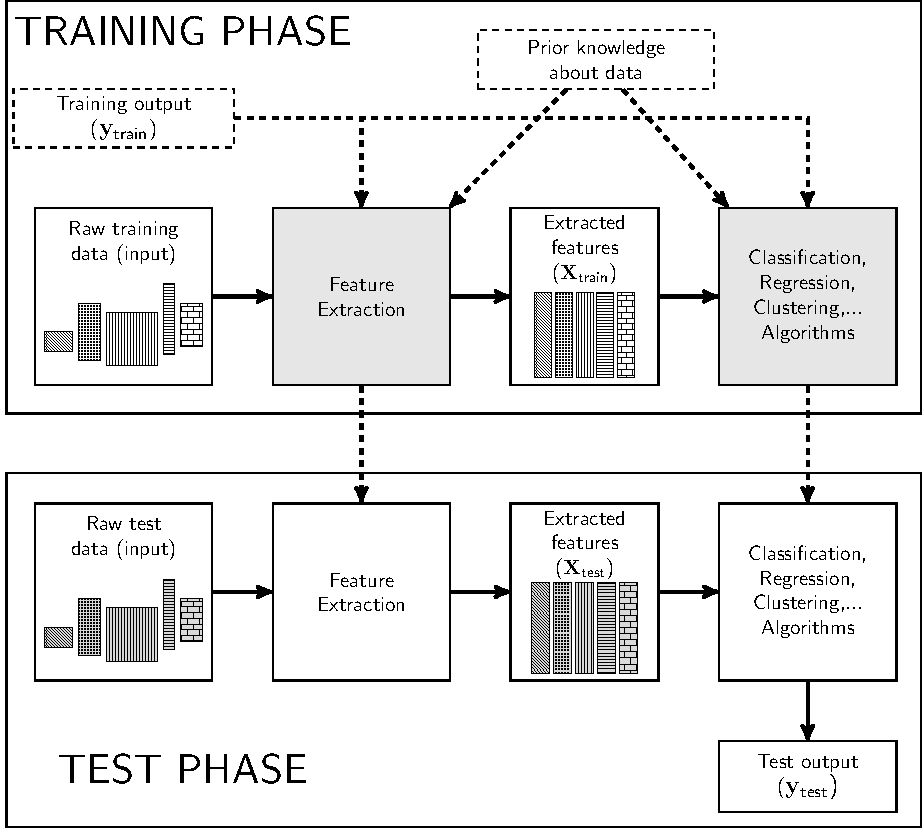
\includegraphics[width = \textwidth]{Chapters/01_Overview/11_featureengineering/latex/ML_models.pdf}
%     \caption[]{Mô hình chung cho các bài toán Machine Learning.}
%     \label{fig:22_1}
% \end{figure}



% Trong Hình \ref{fig:22_1}, phần TRAINING PHASE, chúng ta có thể thấy rằng có hai khối chính là \textit{Feature Extraction} và \textit{Classification/Regression/Clustering...} Các phương pháp \textit{truyền thống} thường xây dựng hai khối này qua các bước riêng rẽ. Phần Feature Extraction với dữ liệu ảnh có thể dùng các feature descriptor như \href{http://opencv-python-tutroals.readthedocs.io/en/latest/py_tutorials/py_feature2d/py_sift_intro/py_sift_intro.html}{SIFT}, \href{http://opencv-python-tutroals.readthedocs.io/en/latest/py_tutorials/py_feature2d/py_surf_intro/py_surf_intro.html}{SURF}, \href{http://www.learnopencv.com/histogram-of-oriented-gradients/}{HOG}; với dữ liệu văn bản thì có thể là \href{http://machinelearningcoban.com2017/02/06/featureengineering/#bag-of-words}{Bag of Words} hoặc \href{http://www.tfidf.com/}{TF-IDF}. Nếu là các bài toán classification, phần còn lại có thể là SVM thông thường hay các bộ phân lớp \textit{truyền thống} khác.

% Với sự phát triển của Deep Learning trong những năm gần đây, người ta cho rằng các hệ thống \textit{end-to-end} (từ đầu đến cuối) mang lại kết quả tốt hơn nhờ và việc các hai khối phía trên được huấn luyện cùng nhau, bổ trợ lẫn nhau. Thực tế cho thấy, các phương pháp \textit{state-of-the-art} thường là các mô hình \textit{end-to-end}.

% Support Vector Machine được chứng minh là nhìn chung tốt hơn Logistic Regression vì chúng có quan tâm đến việc tạo \textit{margin} lớn nhất giữa các classes. Câu hỏi đặt ra là:

% \textbf{Liệu có cách nào giúp kết hợp SVM với Neural Networks để tạo ra một bộ phân lớp tốt với bài toán multi-class classification? Hơn nữa, toàn bộ hệ thống có thể được huấn luyện theo kiểu \textit{end-to-end}?}

% Câu trả lời sẽ được tìm thấy trong bài viết này, bằng một phương pháp được gọi là \textit{Multi-class Support Vector Machine}.

% Và để cho bài viết hấp dẫn hơn, tôi xin giới thiệu luôn, ở phần cuối, chúng ta sẽ cùng lập trình từ đầu đến cuối để giải quyết bài toán phân lớp với bộ cơ sở dữ liệu nổi tiếng: CIFAR10.
Chúng ta sẽ tìm hiểu SVM đa lớp qua ví dụ về bài toán phân loại các bức ảnh thuộc 10 lớp khác nhau trong bộ cơ sở dữ liệu CIFAR10 (\url{https://goo.gl/9KKbQu}).

\subsection{Bộ cơ sở dữ liệu CIFAR10}

Bộ cơ sở dữ liệu CIFAR10 gồm 60000 ảnh có kích thước $32 \times 32$ điểm ảnh
thuộc 10 lớp dữ liệu: \textit{plane, car, bird, cat, deer, dog, frog, horse,
ship, và truck}. Một vài ví dụ của mỗi lớp được hiển thị trong Hình \ref{fig:22_2}.
Tập huấn luyện gồm 50000 bức ảnh, tập kiểm tra gồm 10000 ảnh còn lại.
Trong số 50000 ảnh huấn luyện, 1000 ảnh sẽ được lấy ra ngẫu nhiên làm tập xác
thực.
% ******************************************************************************
\begin{figure}[t]
\centering
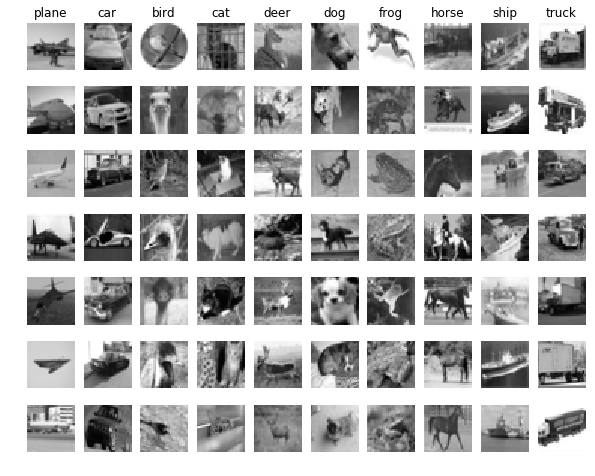
\includegraphics[width = \textwidth]{Chapters/09_SupportVectorMachines/22_multiclasssvm/cifar_gray.png}
\caption[]{Ví dụ về các bức ảnh trong 10 lớp của bộ dữ liệu CIFAR10 (xem ảnh màu tại trang~\pageref{fig:22_2_c}).}
\label{fig:22_2}
\end{figure}
% ******************************************************************************
Đây là một bộ cơ sở dữ liệu tương đối khó vì các bức ảnh có độ phân giải thấp và
các đối tượng trong cùng một lớp biến đổi rất nhiều về màu sắc và hình dáng.
Thuật toán tốt nhất hiện nay cho bài toán này đã đạt được độ chính xác trên 96\%
(\url{https://goo.gl/w1sgK4}), sử dụng một mạng neuron tích chập đa tầng kết hợp
với một hồi quy softmax ở tầng cuối cùng. Trong chương này, chúng ta sẽ sử dụng
một mạng neuron đơn giản với một tầng SVM đa lớp để giải quyết bài toán. Mô hình
này chỉ mang lại độ chính xác khoảng 40\%, nhưng cũng đã rất ấn tượng. Chúng ta
sẽ phân tích mô hình và lập trình chỉ sử dụng thư viện numpy. Bài toán này cũng
như nội dung chính của chương được lấy từ ghi chép bài giảng \textit{Linear
Classifier II  --  CS231n 2016} (\url{https://goo.gl/y3QsDP}) và
\textit{Assignment \#1  --  CS231n 2016} (\url{https://goo.gl/1Qh84b}).

Trước khi đi vào mục xây dựng và tối ưu hàm mất mát cho SVM đa lớp, chúng ta cần xây dựng một bộ trích chọn đặc trưng cho mỗi ảnh.

\subsection{Xây dựng vector đặc trưng}
Sử dung phương pháp xây dựng vector đặc trưng đơn giản nhất: lấy
trực tiếp tất cả các điểm trong mỗi ảnh và chuẩn hóa dữ liệu.
\begin{itemize}
\item Mỗi ảnh {màu} của CIFAR-10 có kích thước đều là $32
\times 32$ điểm ảnh, vì vậy việc đầu tiên chúng ta có thể làm là {kéo dài} cả ba kênh \textit{red, green, blue} của bức ảnh thành một vector có kích thước $3 \times 32 \times 32 = 3072$.

\item Phương pháp chuẩn hóa dữ liệu đơn giản là trừ mỗi vector đặc trưng đi vector trung bình của dữ liệu trong tập huấn luyện. Việc này sẽ giúp tất cả các thành phần đặc trưng có trung bình bằng không trên tập huấn luyện.

\end{itemize}

\subsection{Thủ thuật gộp hệ số điều chỉnh}
\index{thủ thuật gộp hệ số điều chỉnh -- bias trick}
\index{bias trick -- thủ thuật gộp hệ số điều chỉnh}
\begin{figure}[ht]
\centering
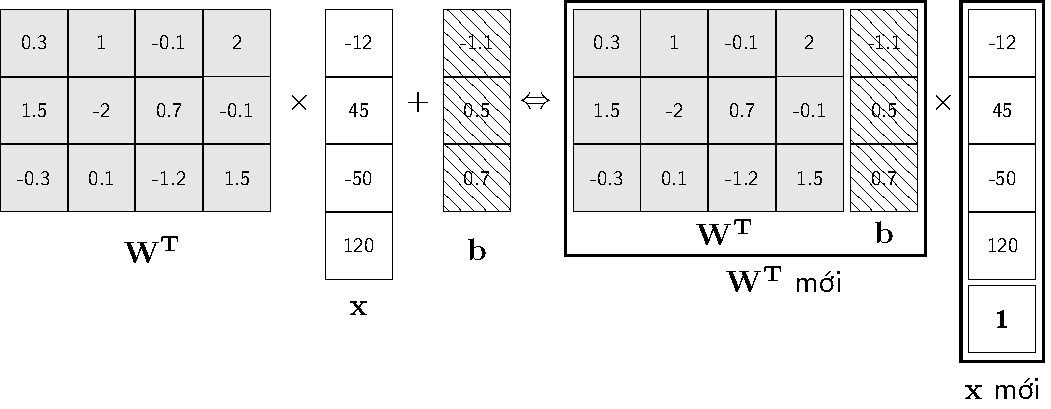
\includegraphics[width = \textwidth]{Chapters/09_SupportVectorMachines/22_multiclasssvm/latex/biastrick.pdf}
\caption[]{Thủ thuật gộp hệ số điều chỉnh}
\label{fig:22_3}
\end{figure}

Với một ma trận trọng số $\mathbf{W} \in \mathbb{R}^{d\times C}$ và vector điều chỉnh $\mathbf{b} \in \mathbb{R}^C$, vector điểm số ứng với một vector đầu vào $\bx$ được tính bởi:
\begin{equation}
\bz = f(\mathbf{x}, \mathbf{W}, \mathbf{b}) = \mathbf{W}^T\mathbf{x} + \mathbf{b}
\end{equation}
Để biểu thức này đơn giản hơn, ta có thể thêm một phần tử bằng một vào $\mathbf{x}$ và {gộp} vector điều chỉnh $\mathbf{b}$ vào ma trận trọng số $\mathbf{W}$
như ví dụ trong Hình \ref{fig:22_3}. Kỹ thuật này được gọi là \textit{thuật gộp hệ số điều chỉnh} (bias trick). Từ đây, khi viết
$\mathbf{W}$ và $\mathbf{x}$, ta ngầm hiểu chúng đã được mở rộng như
phần bên phải của Hình \ref{fig:22_3}.

Tiếp theo, chúng ta viết chương trình lấy dữ liệu từ CIFAR10, chuẩn hoá dữ
liệu và thêm phần tử bằng một vào cuối mỗi vector đặc trưng. Đồng thời, 1000 dữ liệu từ tập huấn luyện cũng được tách ra làm tập xác thực:
% \newpage

\begin{lstlisting}[language=Python]
from __future__ import print_function
import numpy as np
# need cs231 folder from https://goo.gl/cgJgcG
from cs231n.data_utils import load_CIFAR10

# Load CIFAR 10 dataset
cifar10_dir = 'cs231n/datasets/cifar-10-batches-py'
X_train, y_train, X_test, y_test = load_CIFAR10(cifar10_dir)

# Extract a validation from X_train
from sklearn.model_selection import train_test_split
X_train, X_val, y_train, y_val = train_test_split(X_train, y_train, test_size= 1000)

# mean image of all training images
img_mean = np.mean(X_train, axis = 0)

def feature_engineering(X):
    X -= img_mean # zero-centered
    N = X.shape[0] # number of data point
    X = X.reshape(N, -1) # vectorization
    return np.concatenate((X, np.ones((N, 1))), axis = 1) # bias trick

X_train = feature_engineering(X_train)
X_val   = feature_engineering(X_val)
X_test  = feature_engineering(X_test)
print('X_train shape = ', X_train.shape)
print('X_val shape   = ', X_val.shape)
print('X_test shape  = ', X_test.shape)
\end{lstlisting}

\kq
\begin{lstlisting}[language=Python]
X_train shape =  (49000, 3073)
X_val shape   =  (1000, 3073)
X_test shape  =  (10000, 3073)
\end{lstlisting}
\section{Xây dựng hàm mất mát }
% Chúng ta cùng quay lại một chút với ý tưởng của Softmax Regression với hàm mất mát Cross-entropy. Sau đó, chúng ta sẽ làm quen với Multi-class SVM với hàm mất mát hinge loss mở rộng.


% \subsection{Nhắc lại Softmax Regression. }
% Chúng ta cùng xem lại \href{http://machinelearningcoban.com/2017/02/17/softmax/#-softmax-function}{Softmax layer đã được trình bày trong Bài 13}.
% % <hr>
% % <div class="imgcap">
% % <img src ="\assets\13_softmax\softmax_nn.png" align = "center" width = "800">
% % <div class = "thecap">Hình 4: Mô hình Softmax Regression dưới dạng Neural network.</div>
% % </div>
% % <hr>
% \begin{figure}[t]
% \centering
%     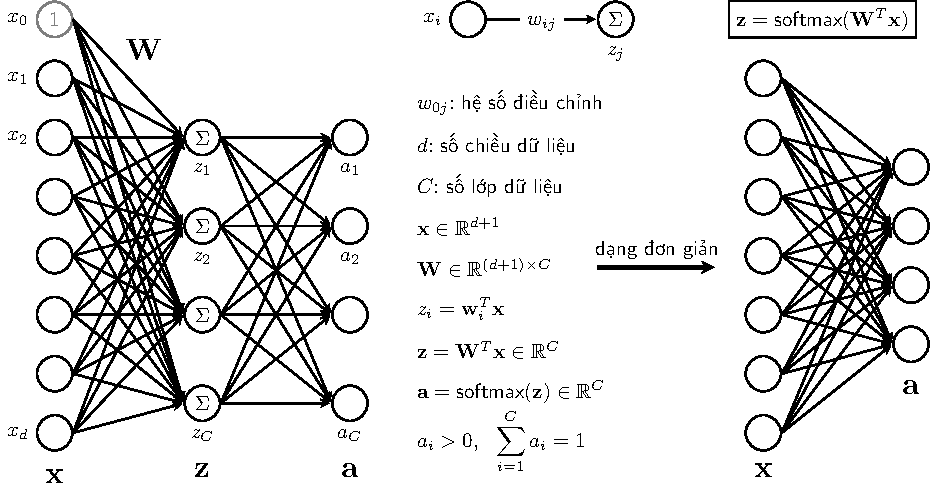
\includegraphics[width = \textwidth]{Chapters/05_NeuralNetworks/13_softmax/latex/softmax_nn.pdf}
%     \caption[]{Mô hình Softmax Regression dưới dạng Neural Network.}
%     \label{fig:22_4}
% \end{figure}


% Trong Hình 4 ở trên, dữ liệu trong lớp màu xanh lục được coi như \textit{feature vector} của dữ liệu. Với dữ liệu CIFAR-10, nếu ta coi mỗi feature là giá trị của từng pixel trong ảnh, tổng số chiều của \textit{feature vector} cho mỗi bức ảnh là $32\times 32 \times 3 +1 = 3073$, với 3 là số channels trong bức ảnh (Red, Green, Blue).

% Qua ma trận hệ số $\mathbf{W}$, dữ liệu ban đầu trở thành $\mathbf{z} = \mathbf{W}^T\mathbf{x}$.

% Lúc này, ứng với mỗi một trong $C$ classes, chúng ta nhận được một giá trị tương ứng $z_i$ ứng với class thứ $i$. Giá trị $z_i$ này còn được gọi là \textit{score} của dữ liệu $\mathbf{x}$ ứng với class thứ $i$.

% Ý tưởng chính trong Sofftmax Regression là đi tìm ma trận hệ số $\mathbf{W}$, mỗi cột của ma trận này ứng với một class, sao cho \textit{score vector} $\mathbf{z}$ đạt giá trị lớn nhất tại phần tử tương ứng với class chính xác của nó. Sau khi mô hình đã được \textit{trained}, \textit{nhãn} của một điểm dữ liệu mới được tính là vị trí của thành phần score có giá trị lớn nhất trong \textit{score vector}. Xem ví dụ trong Hình 5 dưới đây:

% <hr>
% <div class="imgcap">
% <img src ="\assets\22_multiclasssvm\scores.png" align = "center" width = "800">
% <div class = "thecap">Hình 5: Ví dụ về cách tính score vector. Khi test, nhãn của dữ liệu được xác định dựa trên class có score cao nhất.</div>
% </div>
% <hr>

\begin{figure}[t]
\centering
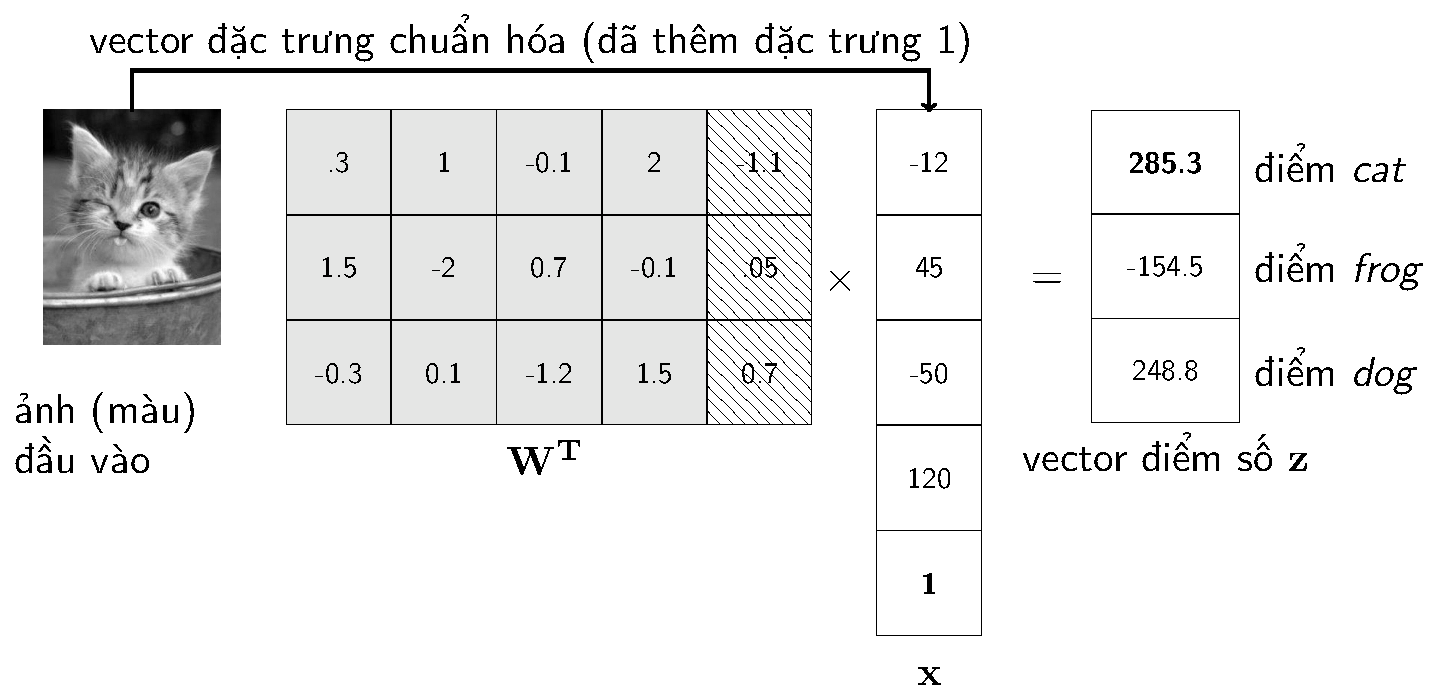
\includegraphics[width = .8\textwidth]{Chapters/09_SupportVectorMachines/22_multiclasssvm/latex/scores.pdf}
\caption[]{Ví dụ về cách tính vector điểm số. Nhãn của một điểm dữ liệu được xác định dựa trên lớp tương ứng có điểm cao nhất.}
\label{fig:22_5}
\end{figure}

% Để huấn luyện trên tập các cặp (\textit{dữ liệu}, \textit{nhãn}), Softmax Regression sử dụng hàm softmax để đưa \textit{score vector} về dạng phân phối xác suất có các phần tử là dương và có tổng bằng 1. Sau đó dùng hàm cross entropy để \textit{ép} vector xác suất này gần với vector xác suất \textit{thật sự} của dữ liệu - tức one-hot vector mà chỉ có đúng 1 phần tử bằng 1 tại class tương ứng, các phần tử còn lại bằng 0.


\subsection{Mất mát bản lề tổng quát cho SVM đa lớp}
\index{mất mát bản lề tổng quát}
Trong SVM đa lớp, nhãn của một điểm dữ liệu mới được xác định bởi thành phần có
giá trị lớn nhất trong vector điểm số $\bz = \bW^T\bx$ (xem
Hình~\ref{fig:22_5}). Điều này tương tự như hồi quy softmax. Hồi quy softmax sử
dụng mất mát entropy chéo để \textit{ép} hai vector xác suất bằng nhau. Việc tối
thiểu mất mát entropy chéo tương đương với việc ép phần tử tương ứng {nhãn}
thực sự trong vector xác suất gần bằng một, đồng thời khiến các phần tử xác suất
còn lại gần bằng không. Điều này khiến  phần tử tương ứng với nhãn thực sự càng
lớn hơn các phần tử còn lại càng tốt. SVM đa lớp sử dụng một giải pháp khác cho
{mục đích tương tự}.

Trong SVM đa lớp, hàm mất mát được xây dựng dựa trên định nghĩa của vùng an toàn
giống như SVM lề cứng/mềm cho bài toán phân loại nhị phân. Cụ thể, SVM đa lớp ép
thành phần ứng của nhãn thực sự của vector điểm số lớn hơn các phần tử khác;
không những thế, nó cần lớn hơn một đại lượng $\Delta > 0$ như được mô tả trong
Hình~\ref{fig:22_6}. Ta gọi đại lượng $\Delta$ này là \textit{lề an toàn}.

% ******************************************************************************
\begin{figure}[t]
\centering
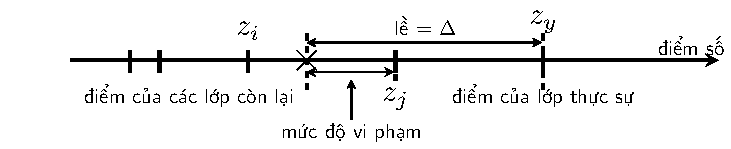
\includegraphics[width
=.85\textwidth]{Chapters/09_SupportVectorMachines/22_multiclasssvm/latex/hinge2.pdf}
\caption[]{Mô tả mất mát bản lề tổng quát. SVM đa lớp ép điểm số của lớp thực sự ($z_y$) cao hơn các điểm số khác
($z_i$) một khoảng cách an toàn $\Delta$. Những điểm số nằm trong vùng an toàn, tức phía trái của điểm $\times$, sẽ gây ra mất mát bằng không. Trong khi đó, những điểm số nằm bên phải điểm $\times$ đã rơi vào vùng không an toàn và cần được gán mất mát dương.}
\label{fig:22_6}
\end{figure}
% ******************************************************************************

Nếu điểm số tương ứng với nhãn thực sự lớn hơn các điểm số khác một lượng bằng
lề an toàn $\Delta$ thì mất mát bằng không. Nói các khác, những điểm số nằm bên
trái điểm $\times$ không gây ra mất mát nào. Ngược lại, các điểm số nằm bên phải
của $\times$ cần bị \textit{xử phạt}, và mức xử phạt tỉ lệ thuận với độ vi
phạm (mức độ vượt quá ranh giới an toàn $\times$).

Để mô tả các mức vi phạm này dưới dạng toán học, trước hết ta giả sử rằng các
thành phần của vector điểm số và các lớp dữ liệu được đánh số thứ tự từ một thay
vì không như hồi quy softmax. Giả sử rằng điểm dữ liệu $\mathbf{x}$ đang xét có
nhãn $y$ và vector điểm số $\mathbf{z} = \bW^T\bx$. Như vậy, điểm số của nhãn
thực sự là $z_y$, điểm số của các nhãn khác là các $z_i, i \neq y$. Trong
Hình~\ref{fig:22_6}, điểm số $z_i$ nằm trong vùng an toàn còn $z_j$ nằm trong
vùng không an toàn. Với mỗi điểm số $z_i$ trong vùng an toàn, mất mát bằng
không. Với mỗi điểm số $z_j$ vượt quá $\times$, mất mát được tính bằng khoảng
cách từ điểm đó tới $\times$: $z_j - (z_y - \Delta) =
\Delta - z_y + z_j$.

% Một cách đơn giản để xác định \textit{loss} như sau:

% \begin{itemize}
%     \item Với mỗi score $z_i$ trong vùng an toàn, \textit{loss} bằng 0.

%     \item Với mỗi socre $z_j$ vượt quá điểm an toàn (điểm $\times$),
%     \textit{loss} do nó gây ra được tính bằng lượng vượt quá so với điểm
%     $\times$ đó, đại lượng này có thể tính được là $z_j - (z_y - \Delta) =
%     \Delta - z_y + z_j$.
% \end{itemize}
Tóm lại, với một điểm số $z_j, j \neq y$, mất mát do nó gây ra là
\begin{equation}
\label{eqn:22_1}
\max(0, \Delta - z_y + z_j) = \max(0, \Delta - \mathbf{w}_y^T\mathbf{x} + \mathbf{w}_j^T\mathbf{x})
\end{equation}
trong đó $\mathbf{w}_j$ là {cột} thứ $j$ của ma trận trọng số $\mathbf{W}$.
Như vậy, mất mát tại một điểm dữ liệu $\mathbf{x}_n, n = 1, 2, \dots, N$ vỡi nhãn $y_n$ là
\begin{equation*}
\mathcal{L}_n = \sum_{j \neq y_n} \max(0, \Delta  - z_{y_n}^n + z_j^n)
\end{equation*}
với $\mathbf{z}^n = \mathbf{W}^T\mathbf{x}_n = [z^n_1, z^n_2, \dots,
z^n_C]^T \in \mathbb{R}^{C \times 1}$ là vector điểm số tương ứng với $\mathbf{x}_n$.
Mất mát trên toàn bộ dữ liệu huấn luyện $\mathbf{X} = [\mathbf{x}_1, \mathbf{x}_2, \dots,
\mathbf{x}_N ]$, mát mát được định nghĩa là
\begin{equation}
\label{eqn:22_2}
\mathcal{L}(\mathbf{X}, \mathbf{y}, \mathbf{W}) = \frac{1}{N}\sum_{n=1}^N \sum_{j \neq y_n} \max(0, \Delta - z_{y_n}^n + z_j^n).
\end{equation}
Trong đó, $\mathbf{y} = [y_1, y_2, \dots, y_N]$ là vector chứa nhãn thực sự
của dữ liệu huấn luyện.

% Có một \textit{bug} trong lỗi này, chúng ta cùng phân tích tiếp.


\subsection{Cơ chế kiểm soát}
\index{suy giảm trọng số -- weight decay}
\index{weight decay -- suy giảm trọng số}
\index{xác thực -- validation!xác thực chéo -- cross-validation}
\index{validation -- xác thực!cross-validation -- xác thực chéo}
\index{cơ chế kiểm soát -- regularization}
\index{regularization -- cơ chế kiểm soát}
Điều gì sẽ xảy ra nếu nghiệm tìm được $\mathbf{W}$ là một nghiệm hoàn hảo, tức không có điểm số nào {vi phạm} và hàm mất mát~\eqref{eqn:22_2}
bằng không? Nói cách khác,
\begin{equation*}
\Delta - z_{y_n}^n + z_j^n   \leq 0 \Leftrightarrow \Delta \leq \mathbf{w}_{y_n}^T \mathbf{x}_n - \mathbf{w}_j^T\mathbf{x}_n~\forall n = 1, 2, \dots, N; j = 1, 2, \dots, C; j \neq y_n
\end{equation*}
Điều này có nghĩa $k\mathbf{W}$ cũng là một nghiệm của bài toán với $k > 1$
bất kỳ. Điều này dẫn tới bài toán có vô số nghiệm và có thể có nghiệm lớn vô cùng. Phương pháp suy giảm trọng số có thể ngăn chặn việc $\mathbf{W}$ trở nên quá lớn:
\begin{equation}
\label{eqn:22_3}
\mathcal{L}(\mathbf{X}, \mathbf{y}, \mathbf{W}) = \underbrace{\frac{1}{N}\sum_{n=1}^N \sum_{j \neq y_n} \max(0, \Delta - \mathbf{w}_{y_n}^T \mathbf{x}_n + \mathbf{w}_j^T\mathbf{x}_n)}_{\text{mất mát dữ liệu}} + \underbrace{\frac{\lambda}{2} \|\mathbf{W}\|_F^2}_{\text{suy giảm trọng số}}
\end{equation}
với $\lambda$ là một tham số kiểm soát dương giúp cân bằng giữa thành phần mất
mát dữ liệu và thành phần kiểm soát. Tham số kiểm soát này được chọn bằng xác
thực chéo.

\subsection{Hàm mất mát của SVM đa lớp}

Có hai siêu tham số trong hàm mất mát \eqref{eqn:22_3} là $\Delta$ và $\lambda$,
câu hỏi đặt ra là làm thế nào để chọn ra cặp giá trị hợp lý nhất cho từng bài
toán. Liệu chúng ta có cần thực hiện xác thực chéo cho từng giá trị không? Trên thực
tế, người ta nhận thấy rằng $\Delta$ có thể được chọn bằng một mà không làm ảnh
hưởng tới chất lượng của nghiệm (\url{https://goo.gl/NSyfQi}). Từ đó, hàm mất
mát của SVM có dạng
\begin{equation}
\label{eqn:22_4}
\mathcal{L}(\mathbf{X}, \mathbf{y}, \mathbf{W}) = \frac{1}{N}\sum_{n=1}^N \sum_{j \neq y_n} \max(0, 1 - \mathbf{w}_{y_n}^T \mathbf{x}_n + \mathbf{w}_j^T\mathbf{x}_n) + \frac{\lambda}{2} \|\mathbf{W}\|_F^2
\end{equation}
Nghiệm của bài toán tối thiểu hàm mất mát có thể tìm được bằng gradient descent.
Điều này sẽ được thảo luận kỹ trong Mục~\ref{sec:22_3}.

% Chúng ta có một nhận xét thú vị:

\subsection{SVM lề mềm là một trường hợp đặc biệt của SVM đa lớp}
(\textit{Hồi quy logistic là một trường hợp đặc biệt của hồi quy softmax.})

Khi số lớp dữ liệu $C = 2$, tạm bỏ qua mất mát kiểm soát, hàm mất mát tại mỗi điểm dữ liệu trở thành
\begin{equation}
\mathcal{L}_n = \sum_{j \neq y_n} \max(0, 1 - \mathbf{w}_{y_n}^T \mathbf{x}_n + \mathbf{w}_j^T\mathbf{x}_n)
\end{equation}
Xét hai trường hợp:
\begin{itemize}
\item $y_n = 1 \Rightarrow \mathcal{L}_n = \max(0, 1 - \mathbf{w}_1^T\mathbf{x}_n + \mathbf{w}_2^T\mathbf{x}_n) = \max(0, 1 - (1)(\mathbf{w}_1 - \mathbf{w}_2)^T\mathbf{x})$

\item $y_n = 2 \Rightarrow \mathcal{L}_n = \max(0, 1 - \mathbf{w}_2^T\mathbf{x}_n + \mathbf{w}_1^T\mathbf{x}_n) = \max(0, 1 - (-1)(\mathbf{w}_1 - \mathbf{w}_2)^T\mathbf{x})$
\end{itemize}
Nếu ta thay $y_n = -1$ cho dữ liệu thuộc lớp có nhãn bằng 2 và đặt
$\mathbf{\bar{w}} = \mathbf{w}_1 - \mathbf{w}_2$, hai trường hợp trên có thể được viết gọn thành
\begin{equation*}
\mathcal{L}_n = \max(0, 1 - y_n\mathbf{\bar{w}}^T\mathbf{x}_n)
\end{equation*}
Đây chính là mất mát bản lề trong SVM lề mềm. Như vậy, SVM lề mềm là trường hợp đặc biệt của SVM đa lớp khi số lớp dữ liệu $C = 2$.

\section{Tính toán giá trị và gradient của hàm mất mát}
\label{sec:22_3}
% Để tối ưu hàm mất mát, chúng ta sử dụng phương pháp Stochastic Gradient Method. Điều này có nghĩa là chúng ta cần tính gradient tại mỗi vòng lặp. Đồng thời, \textit{loss} sau mỗi vòng lặp cũng cần được tính để kiểm tra liệu thuật toán có hoạt động như ý muốn hay không.
\index{gradient!gradient xấp xỉ -- numerical gradient}
\index{gradient!numerical gradient -- gradient xấp xỉ}
Với những hàm số phức tạp, việc tính toán gradient rất dễ gây ra kết quả không
chính xác. Trước khi thực hiện các thuật toán tối ưu sử dụng gradient, ta cần
đảm bảo sự chính xác của việc tính gradient. Một lần nữa, có thể sử dụng phương pháp xấp xỉ gradient theo định nghĩa. Để thực hiện phương pháp này, chúng ta
cần tính giá trị của hàm mất mát tại một điểm $\bW$ bất kỳ.

% \newnote{}{
Việc tính toán giá trị của hàm mất mát và gradient của nó tại $\bW$ bất kỳ không
những cần sự chính xác mà còn cần được thực hiện một cách hiệu quả. Để đạt được
điều đó, chúng ta sẽ thực hiện từng bước một. Bước thứ nhất phải đảm bảo rằng các
tính toán là {chính xác}, dù cách tính có thể rất chậm. Bước thứ hai là đảm bảo
các phép tính được thực hiện một cách hiệu quả. Hai bước này nên được thực hiện
trên một lượng dữ liệu nhỏ để có thể nhanh chóng có kết quả. Việc tính xấp xỉ
gradient trên dữ liệu lớn thường tốn rất nhiều thời gian vì phải tính giá trị
của hàm số trên từng thành phần của ma trận trọng số $\bW$. Các quy tắc này cũng
được áp dụng với những bài toán tối ưu khác có sử dụng gradient trong quá trình
tìm nghiệm. Hai mục tiếp theo sẽ mô tả hai bước đã nêu ở trên.


\subsection{Tính chính xác}

% \textit{Naive} dịch tạm ra tiếng Việt có nghĩa là \textit{ngây thơ}, hoặc \textit{ngây ngô}. Trong Machine Learning, từ này cũng hay được sử dụng với ý chỉ sự đơn giản.

Dưới đây là cách tính hàm mất mát và gradient trong \eqref{eqn:22_4}
bằng hai vòng \pythoninline{for}:
\begin{lstlisting}[language=Python]
def svm_loss_naive(W, X, y, reg):
    ''' calculate loss and gradient of the loss function at W. Naive way
    W: 2d numpy array of shape (d, C). The weight matrix.
    X: 2d numpy array of shape (N, d). The training data
    y: 1d numpy array of shape (N,). The training label
    reg: a positive number. The regularization parameter
    '''
    d, C = W.shape # data dim, No. classes
    N = X.shape[0] # No. points
    loss = 0
    dW = np.zeros_like(W)
    for n in xrange(N):
        xn = X[n]
        score = xn.dot(W)
        for j in xrange(C):
            if j == y[n]:
                continue
            margin = 1 - score[y[n]] + score[j]
            if margin > 0:
                loss += margin
                dW[:, j] += xn
                dW[:, y[n]] -= xn

    loss /= N
    loss += 0.5*reg*np.sum(W * W) # regularization
    dW /= N
    dW += reg*W
    return loss, dW

# random, small data
d, C, N = 100, 3, 300
reg = .1
W_rand = np.random.randn(d, C)
X_rand = np.random.randn(N, d)
y_rand = np.random.randint(0, C, N)
# sanity check
print('Loss with reg = 0  :', svm_loss_naive(W_rand, X_rand, y_rand, 0)[0])
print('Loss with reg = 0.1:', svm_loss_naive(W_rand, X_rand, y_rand, .1)[0])
\end{lstlisting}
\kq
\begin{lstlisting}
Loss with reg = 0  : 12.5026818221
Loss with reg = 0.1: 27.7805360552
\end{lstlisting}


Cách tính với hai vòng \pythoninline{for} lồng nhau như trên mô tả chính xác
biểu thức~\eqref{eqn:22_4} nên tính chính xác có thể được đảm bảo. Việc kiểm tra ở cuối cho cái nhìn ban đầu về hàm mất
mát: dương và không có kiểm soát sẽ cho giá trị cao hơn.

Cách tính gradient cho phần mất mát dữ liệu dựa trên nhận xét sau
đây:
\begin{eqnarray}
\label{eqn:22_5}
\nabla_{\mathbf{w}_{y_n}}\max(0, 1 - \mathbf{w}_{y_n}^T \mathbf{x}_n + \mathbf{w}_j^T\mathbf{x}_n) &=&
\left\{
\begin{matrix}
0 & \text{nếu}& 1 - \mathbf{w}_{y_n}^T \mathbf{x}_n + \mathbf{w}_j^T\mathbf{x}_n < 0 \\\
-\mathbf{x}_n & \text{nếu} &1 - \mathbf{w}_{y_n}^T \mathbf{x}_n + \mathbf{w}_j^T\mathbf{x}_n > 0
\end{matrix}
\right.\\\
\label{eqn:22_6}
\nabla_{\mathbf{w}_{j}}\max(0, 1 - \mathbf{w}_{j}^T \mathbf{x}_n + \mathbf{w}_j^T\mathbf{x}_n) &=&
\left\{
\begin{matrix}
0 & \text{nếu}& 1 - \mathbf{w}_{y_n}^T \mathbf{x}_n + \mathbf{w}_j^T\mathbf{x}_n < 0 \\\
\mathbf{x}_n & \text{nếu} &1 - \mathbf{w}_{y_n}^T \mathbf{x}_n + \mathbf{w}_j^T\mathbf{x}_n > 0
\end{matrix}
\right.
\end{eqnarray}

Mặc dù gradient không xác định tại các điểm mà $1 - \mathbf{w}_{y_n}^T \mathbf{x}_n + \mathbf{w}_j^T\mathbf{x}_n = 0$, ta vẫn có thể giả sử rằng gradient tại 0 cũng bằng 0.

Việc kiểm tra tính chính xác của gradient bằng phương pháp xấp xỉ gradient theo định nghĩa xin dành lại cho bạn đọc.

Khi tính chính xác của gradient đã được đảm bảo, ta cần một cách hiệu quả để tính gradient.



\subsection{Tính hiệu quả}


\index{vector hóa -- vectorization}
\index{vectorization -- vector hóa}
Cách tính toán hiệu quả thường không chứa các vòng \pythoninline{for} mà được
viết gọn lại sử dụng các kỹ thuật vector hóa. Để dễ hình dung, chúng ta cùng
quan sát Hình \ref{fig:22_7}. Ở đây, chúng ta tạm quên thành phần kiểm soát vì
giá trị và gradient của thành phần này đều được tính một cách đơn giản. Chúng ta cũng
bỏ qua hệ số $\frac{1}{N}$ cho các phép tính đơn giản hơn.


Giả sử có bốn lớp dữ liệu và mini-batch $\bX$ gồm ba điểm dữ liệu $\bX = \bmt
\mathbf{x}_1& \mathbf{x}_2 & \mathbf{x}_3\emt$ lần lượt thuộc các lớp 1, 3, 2
(vector $\by$). Các ô có nền màu xám ở mỗi cột tương ứng với nhãn thực sự của
điểm dữ liệu. Các bước tính giá trị và {gradient} của hàm mất mát có thể được
hình dung như sau:
\begin{itemize}
\item {Bước 1:} Tính ma trận điểm số $\mathbf{Z} = \mathbf{W}^T\mathbf{X}$.

\item {Bước 2:} Với mỗi ô, tính $\max(0, 1 - \mathbf{w}_{y_n}^T
\mathbf{x}_n + \mathbf{w}_j^T\mathbf{x}_n)$. Vì biểu thức hàm mất mát cho một điểm dữ liệu không chứa thành phần $j = y_n$ nên ta không cần tính
các ô có nền màu xám. Sau khi tính được giá trị của từng ô, ta chỉ quan tâm
tới các ô có giá trị lớn hơn 0 -- các ô có nền sọc chéo. Lấy tổng tất cả các
phần tử của các ô nền sọc chéo, ta được giá trị của hàm mất mát. Ví dụ, nhìn
vào ma trận ở giữa trong Hình~\ref{fig:22_7}, giá trị hàng thứ hai, cột
thứ nhất bằng $\max(0, 1 - 2 + 1.5) = \max(0, 0.5) = 0.5$. Giá trị hàng
thứ ba, cột thứ nhất bằng $\max(0, 1 -2 + (-0.2)) = \max(0, -1.2) = 0$. Giá
trị hàng thứ tư, cột thứ nhất bằng $\max(0, 1 - 2 + 1.7) = 0.7$. Tương tự
với các cột còn lại.

\item {Bước 3:} Theo công thức~\eqref{eqn:22_5} và~\eqref{eqn:22_6},
với ô nền sọc ở hàng thứ hai, cột thứ nhất (ứng với điểm dữ liệu $\bx_1$),
gradient theo vector trọng số $\mathbf{w}_2$ được cộng thêm một lượng
$\mathbf{x}_1$ và gradient theo vector trọng số $\mathbf{w}_1$ bị trừ đi một
lượng $\mathbf{x}_1$. Như vậy, trong cột thứ nhất, có bao nhiêu ô nền sọc
thì có bấy nhiêu lần gradient của $\mathbf{w}_1$ bị trừ đi một lượng
$\mathbf{x}_1$. Xét ma trận bên phải, giá trị của ô ở hàng thứ $i$, cột thứ
$j$ là hệ số của gradient theo $\bw_i$ gây ra bởi điểm dữ liệu $\bx_j$. Tất
cả các ô nền sọc đều có giá trị bằng 1. Ô màu xám ở cột thứ nhất phải bằng
-2 vì cột đó có hai ô nền sọc. Tương tự với các ô nền sọc và xám còn lại.

\item {Bước 4:} Cộng theo mỗi hàng, ta được gradient theo
hệ số của lớp tương ứng.
\end{itemize}
% ******************************************************************************
\begin{figure}[t]
\centering
% 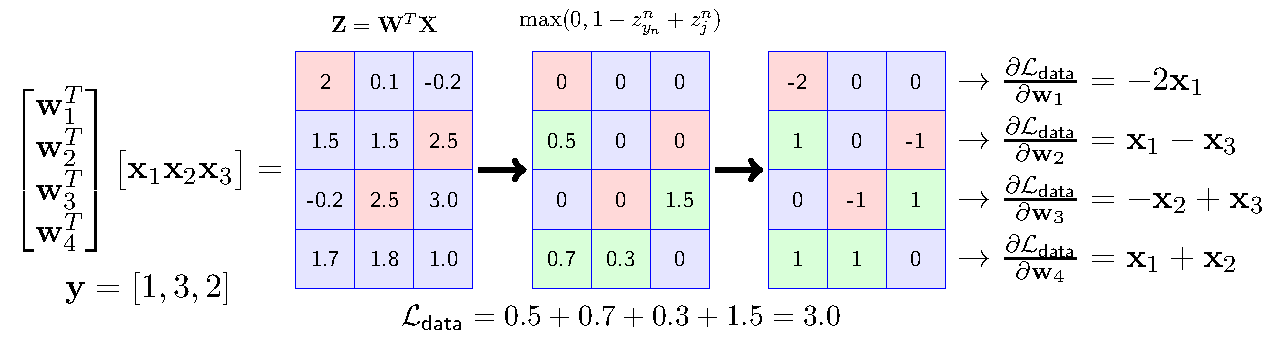
\includegraphics[width = \textwidth]{Chapters/09_SupportVectorMachines/22_multiclasssvm/latex/vectorized_loss.pdf}
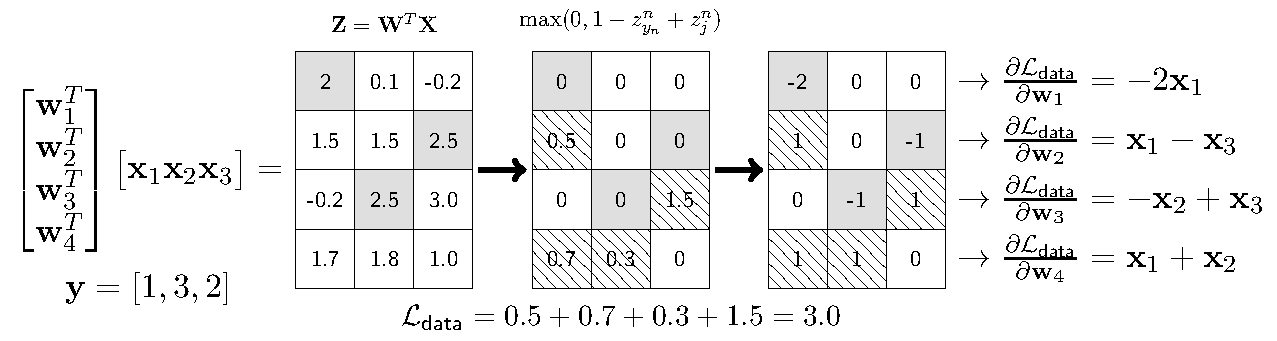
\includegraphics[width = \textwidth]{Chapters/09_SupportVectorMachines/22_multiclasssvm/latex/vectorized_loss_gray.pdf}
\caption[]{Mô phỏng cách tính hàm mất mát và gradient trong SVM đa lớp.} \label{fig:22_7}
\end{figure}
% ******************************************************************************

Cách tính toán trên đây có thể thực hiện như sau:

% \newpage
\begin{lstlisting}[language=Python]
def svm_loss_vectorized(W, X, y, reg):
    d, C = W.shape
    N = X.shape[0]
    loss = 0
    dW = np.zeros_like(W)
    Z = X.dot(W) # shape (N, C)
    id0 = np.arange(Z.shape[0])
    correct_class_score = Z[id0, y].reshape(N, 1) # shape (N, 1)
    margins = np.maximum(0, Z - correct_class_score + 1) # shape (N, C)
    margins[id0, y] = 0
    loss = np.sum(margins)
    loss /= N
    loss += 0.5 * reg * np.sum(W * W)

    F = (margins > 0).astype(int)# shape (N, C)
    F[np.arange(F.shape[0]), y] = np.sum(-F, axis = 1)
    dW = X.T.dot(F)/N + reg*W
    return loss, dW
\end{lstlisting}

Đoạn mã phía trên không chứa vòng \pythoninline{for} nào. Để kiểm tra tính
chính xác và hiệu quả của hàm này, chúng ta cần kiểm chứng ba điều. (i) Giá trị
hàm mất mát đã chính xác? (ii) Giá trị gradient đã chính xác? (iii)
Cách tính đã thực sự hiệu quả?:
% \newpage
\begin{lstlisting}[language=Python]
d, C = 3073, 10
W_rand = np.random.randn(d, C)
import time
t1 = time.time()
l1, dW1 = svm_loss_naive(W_rand, X_train, y_train, reg)
t2 = time.time()
l2, dW2 = svm_loss_vectorized(W_rand, X_train, y_train, reg)
t3 = time.time()
print('Naive       --  run time:', t2 - t1, '(s)')
print('Vectorized  --  run time:', t3 - t2, '(s)')
print('loss difference:', np.linalg.norm(l1 - l2))
print('gradient difference:', np.linalg.norm(dW1 - dW2))
\end{lstlisting}
\kq
\begin{lstlisting}
Naive       --  run time: 7.34640693665 (s)
Vectorized  --  run time: 0.365024089813 (s)
loss difference: 8.73114913702e-11
gradient difference: 1.87942037251e-10
\end{lstlisting}
Kết quả cho thấy cách tính vector hóa hiệu quả hơn khoảng 20 lần và sự chênh lệch giữa hai cách tính là không đáng kể.
Như vậy cả tính chính xác và tính hiệu quả đều đã được đảm bảo.

\subsection{Mini-batch gradient descent cho SVM đa lớp}

Việc huấn luyện SVM đa lớp có thể thực hiện như sau:
\begin{lstlisting}[language=Python]
def multiclass_svm_GD(X, y, Winit, reg, lr=.1,
                      batch_size = 1000, num_iters = 50, print_every = 10):
    W = Winit
    loss_history = []
    for it in xrange(num_iters):
        mix_ids = np.random.permutation(X.shape[0])
        n_batches = int(np.ceil(X.shape[0]/float(batch_size)))
        for ib in range(n_batches):
            ids = mix_ids[batch_size*ib: min(batch_size*(ib+1), X.shape[0])]
            X_batch = X[ids]
            y_batch = y[ids]
            lossib, dW = svm_loss_vectorized(W, X_batch, y_batch, reg)
            loss_history.append(lossib)
            W -= lr*dW
        if it % print_every == 0 and it > 0:
            print('it %d/%d, loss = %f' %(it, num_iters, loss_history[it]))
    return W, loss_history
\end{lstlisting}
\begin{lstlisting}[language=Python]
d, C = X_train.shape[1], 10
reg = .1
W = 0.00001*np.random.randn(d, C)

W, loss_history = multiclass_svm_GD(X_train, y_train, W, reg, lr = 1e-8, num_iters = 50, print_every = 5)
\end{lstlisting}
\kq
\begin{lstlisting}
epoch 5/50, loss = 5.482782
epoch 10/50, loss = 5.204365
epoch 15/50, loss = 4.885159
epoch 20/50, loss = 5.051539
epoch 25/50, loss = 5.060423
epoch 30/50, loss = 4.691241
epoch 35/50, loss = 4.841132
epoch 40/50, loss = 4.643097
epoch 45/50, loss = 4.691177
\end{lstlisting}
Ta thấy rằng giá trị hàm mất mát có xu hướng giảm và hội tụ nhanh. Giá trị hàm mất mát sau mỗi vòng lặp được minh hoạ trong Hình~\ref{fig:22_8}.
% ******************************************************************************
\begin{figure}[t]
% caption on side

\floatbox[{\capbeside\thisfloatsetup{capbesideposition={right,top},capbesidewidth=5cm}}]{figure}[\FBwidth]
{\caption{
Lịch sử giá trị hàm mất mát qua các vòng lặp. Ta thấy rằng mất mát có xu hướng giảm và hội tụ khá nhanh.
}
\label{fig:22_8}}
{ % figure here
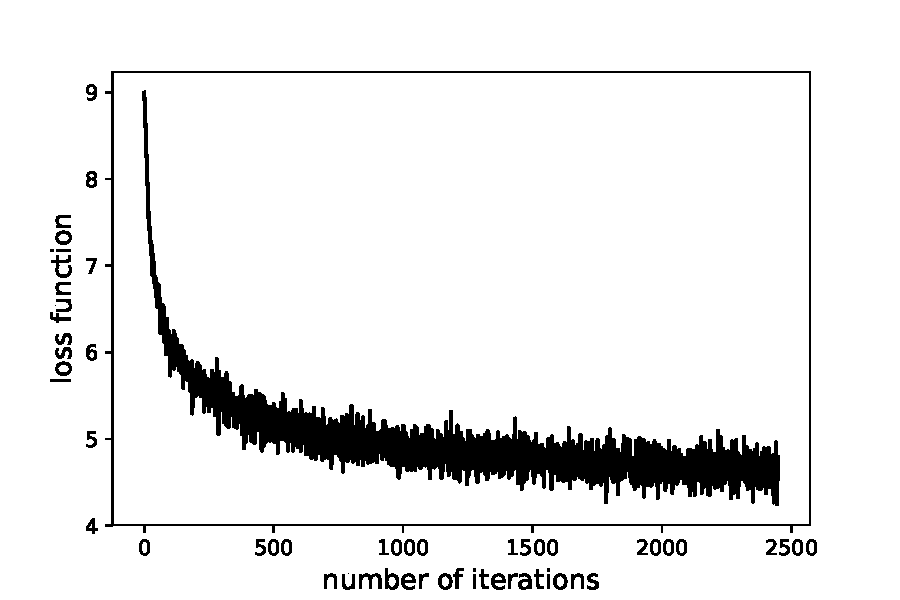
\includegraphics[width=.65\textwidth]{ebookML_src/src/multiclasssvm/loss_history.pdf}
}
\end{figure}
% ******************************************************************************

Sau khi đã tìm được ma trận trọng số $\bW$,
chúng ta cần viết các hàm xác định nhãn của các điểm dữ liệu mới và đánh giá độ chính xác của mô hình:
\begin{lstlisting}[language=Python]
def multisvm_predict(W, X):
    Z = X.dot(W)
    return np.argmax(Z, axis=1)

def evaluate(W, X, y):
    y_pred = multisvm_predict(W, X)
    acc = 100*np.mean(y_pred == y)
    return acc
\end{lstlisting}

\index{tìm trên lưới -- grid search}
\index{grid search -- tìm trên lưới}
Tiếp theo, ta sử dụng tập xác thực để chọn ra bộ siêu tham số mô hình phù
hợp. Có hai siêu tham số trong thuật toán tối ưu SVM đa lớp: tham số kiểm soát và tốc độ học. Hai tham số này sẽ được tìm
bằng phương pháp \textit{tìm trên lưới} (grid search). Bộ giá trị mang lại độ chính xác trên tập xác thực cao nhất sẽ được dùng để đánh giá tập kiểm tra:
\begin{lstlisting}[language=Python]
lrs = [1e-9, 1e-8, 1e-7, 1e-6]
regs = [0.1, 0.01, 0.001, 0.0001]
best_W = 0
best_acc = 0
for lr in lrs:
    for reg in regs:
        W, loss_history = multiclass_svm_GD(X_train, y_train, W, reg, \
                lr = 1e-8, num_iters = 100, print_every = 1e20)
        acc = evaluate(W, X_val, y_val)
        print('lr = %e, reg = %e, loss = %f, val acc = %.2f'
              %(lr, reg, loss_history[-1], acc))
        if acc > best_acc:
            best_acc, best_W = acc, W
\end{lstlisting}
% \newpage
\kq
\begin{lstlisting}[language=Python]
lr = 1.000000e-09, reg = 1.000000e-01, loss = 4.422479, val acc = 40.30
lr = 1.000000e-09, reg = 1.000000e-02, loss = 4.474095, val acc = 40.70
lr = 1.000000e-09, reg = 1.000000e-03, loss = 4.240144, val acc = 40.90
lr = 1.000000e-09, reg = 1.000000e-04, loss = 4.257436, val acc = 41.40
lr = 1.000000e-08, reg = 1.000000e-01, loss = 4.482856, val acc = 41.50
lr = 1.000000e-08, reg = 1.000000e-02, loss = 4.036566, val acc = 41.40
lr = 1.000000e-08, reg = 1.000000e-03, loss = 4.085053, val acc = 41.00
lr = 1.000000e-08, reg = 1.000000e-04, loss = 3.891934, val acc = 41.40
lr = 1.000000e-07, reg = 1.000000e-01, loss = 3.947408, val acc = 41.50
lr = 1.000000e-07, reg = 1.000000e-02, loss = 4.088984, val acc = 41.90
lr = 1.000000e-07, reg = 1.000000e-03, loss = 4.073365, val acc = 41.70
lr = 1.000000e-07, reg = 1.000000e-04, loss = 4.006863, val acc = 41.80
lr = 1.000000e-06, reg = 1.000000e-01, loss = 3.851727, val acc = 41.90
lr = 1.000000e-06, reg = 1.000000e-02, loss = 3.941015, val acc = 41.80
lr = 1.000000e-06, reg = 1.000000e-03, loss = 3.995598, val acc = 41.60
lr = 1.000000e-06, reg = 1.000000e-04, loss = 3.857822, val acc = 41.80
\end{lstlisting}
Như vậy, độ chính xác cao nhất cho tập xác thực là 41.9\%. Ma trận trọng số $\bW$
tốt nhất đã được lưu trong biến \pythoninline{best_W}. Áp dụng mô hình này lên
tập kiểm tra:
\begin{lstlisting}[language=Python]
acc = evaluate(best_W, X_test, y_test)
print('Accuracy on test data = %2f %%'%acc)
\end{lstlisting}
\kq
\begin{lstlisting}[language=Python]
Accuracy on test data =  39.88 %
\end{lstlisting}
Như vậy, kết quả đạt được rơi vào khoảng gần 40 \%.

% Phần code còn lại để giải quyết bài toán phân loại cho cơ sở dữ liệu
% CIFAR-10 có thể tìm thấy trong \href{https://github.com/tiepvupsu/CS231n_2016/blob/master/assignment1/svm.ipynb}{ipython notebook này}.

% (\textit{đây chính là lời giải của tôi cho Assignment \#1 của CS231n, Winter 2016, Stanford.})

% Kết quả đạt được cho CIFAR-10 là khoảng 40\%. Như thế là đã rất tốt với một bài toán khó với 10 classes như thế này, nhất là khi chúng ta chưa phải làm thêm bước feature engineering phức tạp nào. Kết quả của Softmax Regression là khoảng 35\%, các bạn cũng có thể tìm thấy \href{https://github.com/tiepvupsu/CS231n_2016/blob/master/assignment1/softmax.ipynb}{source code tại đây}.


% \textbf{Chú ý:} Trong các bài tập này, dữ liệu được tính toán theo dạng hàng, tức mỗi hàng của $\mathbf{X}$ là một điểm dữ liệu. Khi đó, \textit{score} được tính theo công thức: $\mathbf{Z} = \mathbf{XW}$. Các phép biến đổi có khác một chút so với trường hợp dữ liệu ở dạng cột. Hy vọng các bạn không gặp khó khăn nhiều.


\subsection{Minh họa nghiệm tìm được}

Để ý rằng mỗi $\mathbf{w}_i$ có chiều bằng chiều của dữ liệu. Bằng cách loại bỏ các hệ số điều chỉnh ở cuối và sắp xếp lại các điểm ảnh của mỗi trong
10 vector trọng số tìm được, ta sẽ thu được các {bức ảnh} có cùng kích
thước $3\times 32\times32$ như mỗi ảnh nhỏ trong cơ sở dữ liệu.
Hình~\ref{fig:22_9} minh họa các vector trọng số $\mathbf{w}_i$ tìm được.
% ******************************************************************************
\begin{figure}[t]
\centering
% 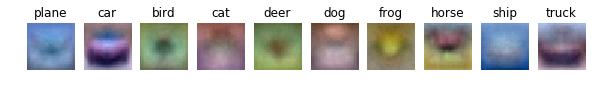
\includegraphics[width = \textwidth]{Chapters/09_SupportVectorMachines/22_multiclasssvm/learned_ws_2.png}
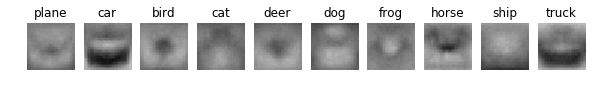
\includegraphics[width = \textwidth]{Chapters/09_SupportVectorMachines/22_multiclasssvm/learned_ws_2_gray.png}
\caption[]{ Minh họa hệ số tìm được dưới dạng các bức ảnh (xem ảnh màu tại trang~\pageref{fig:22_9_c}).}
\label{fig:22_9}
\end{figure}
% ******************************************************************************

Ta thấy rằng vector trọng số tương ứng với mỗi lớp khá giống các bức
ảnh trong lớp đó, ví dụ \textit{car} và \textit{truck}. Vector trọng số của
\textit{ship} và \textit{plane} có mang màu xanh của nước biển và bầu trời (xem
ảnh màu tại trang~\pageref{fig:22_9_c}). Trong khi đó, \textit{horse} giống như
một con ngựa hai đầu; điều này dễ hiểu vì các con ngựa có
thể quay đầu về hai phía trong tập huấn luyện. Có thể nói rằng các hệ số tìm được là ảnh đại diện của mỗi lớp.

Xin nhắc lại, nhãn của mỗi điểm dữ liệu được xác định bởi vị trí của thành phần có giá trị cao nhất trong vector điểm số $\bz = \mathbf{W}^T\mathbf{x}$:
\begin{equation*}
\text{class}(\mathbf{x}) = \arg\max_{i = 1, 2, \dots, C} \mathbf{w}_i^T\mathbf{x}
\end{equation*}
Để ý rằng tích vô hướng chính là đại lượng đo sự tương quan giữa hai vector. Đại
lượng này càng lớn thì sự tương quan càng cao, tức hai vector càng giống nhau.
Như vậy, việc đi tìm nhãn của một bức ảnh mới chính là việc đi tìm bức ảnh đó
giống với bức ảnh {đại diện} cho lớp nào nhất. Kỹ thuật này này khá giống
với KNN, nhưng chỉ có 10 tích vô hướng cần được tính thay vì khoảng cách tới mọi điểm dữ liệu huấn luyện.


\section{Thảo luận }
\begin{itemize}
\item Giống như hồi quy softmax, SVM đa lớp vẫn được coi là một bộ
phân loại tuyến tính vì đường ranh giới giữa các lớp là các đường tuyến tính.

\item SVM hạt nhân hoạt động khá tốt, nhưng việc tính toán ma trận hạt nhân có thể tốn nhiều thời gian và bộ nhớ. Hơn nữa, việc mở rộng SVM hạt nhân cho bài toán phân loại đa lớp thường không hiệu quả bằng SVM đa lớp
vì kỹ thuật được sử dụng vẫn là one-vs-rest. Một ưu điểm nữa của     SVM đa lớp là nó có thể được tối ưu bằng các phương pháp gradient descent, phù hợp
với các bài toán với dữ liệu lớn. Ngoài ra, SVM đa lớp có thể được kết hợp với các mạng neuron đa tầng trong trường hợp dữ liệu không tách biệt tuyến tính.

% \item Có một số phương pháp khác mở rộng mất mát bản lề cho bài toán phân loại đa lớp: $\max(0, 1 - \mathbf{w}_{y_n}^T\mathbf{x}_n + \max_{j \neq y_n}\mathbf{w}_{j}^T\mathbf{x}_n)$. Đây chính là \textit{vi phạm lớn nhất}, so với \textit{tổng vi pham} mà chúng ta sử dụng trong bài này.

\item  Trên thực tế, SVM đa lớp và hồi quy softmax có hiệu quả tương
đương nhau (xem \url{https://goo.gl/xLccj3}). Có thể trong một bài toán cụ
thể, phương pháp này tốt hơn phương pháp kia nhưng điều ngược lại xảy ra
trong các bài toán khác. Khi thực hành, ta có thể thử cả hai
phương pháp rồi chọn phương pháp cho kết quả tốt hơn.
\end{itemize}




% \section{Tài liệu tham khảo }

% [1] \href{http://cs231n.github.io/linear-classify/}{CS231n Convolutional Neural Networks for Visual Recognition}

% [2] \href{https://en.wikipedia.org/wiki/Hinge_loss}{Hinge loss - Wikipedia}
